\documentclass[11pt]{article}
\usepackage[margin=2.2cm]{geometry}
\usepackage{amsmath,amssymb}
\usepackage{graphicx}
\usepackage{booktabs}
\usepackage{hyperref}
\usepackage{caption}
\usepackage{authblk}
\usepackage{titlesec}
\usepackage{xcolor}

\titlespacing*{\section}{0pt}{12pt}{6pt}
\titlespacing*{\subsection}{0pt}{8pt}{4pt}
\hypersetup{colorlinks=true, linkcolor=blue, citecolor=blue, urlcolor=blue}

\title{\vspace{-1.5em}Lévy Process Models for NEPSE Equity Returns:\\
\large Calibration and Forward Simulation for SY Panel Nepal Limited (SYPNL)}
\author[1]{Nabin Pandey}
\affil[1]{Department of Physics, Tri-Chandra Multiple Campus, Tribhuvan University, Kathmandu, Nepal}
\date{\today}

\begin{document}
\maketitle
\vspace{-1.5em}

\begin{abstract}
\noindent We model the daily log-returns of SY Panel Nepal Limited (SYPNL), a stock listed on the Nepal Stock Exchange (NEPSE) on December 10, 2025, using three canonical Lévy process specifications: Merton jump-diffusion, the Variance Gamma (VG) process, and an $\alpha$-stable process. All three arise as special cases of the Lévy--Khintchine decomposition of a general Lévy process into drift, diffusion, and jump components. Parameters are calibrated to the empirical cumulants (and, for the $\alpha$-stable case, by maximum likelihood) of daily log-returns, and the fitted processes are used to Monte Carlo simulate a 30-trading-day forward price distribution. We find broad qualitative agreement across the three models on the shape of the forecast distribution, while noting that the short trading history and non-stationary listing-rally period impose significant limits on calibration reliability.
\end{abstract}

\section{Introduction}
A Lévy process $\{X_t\}_{t\ge 0}$ is a stochastically continuous process with independent, stationary increments. Every such process decomposes, via the Lévy--Khintchine formula, into a deterministic drift, a Brownian (diffusive) component, and a jump component governed by a Lévy measure $\nu$:
\begin{equation}
\mathbb{E}\left[e^{iuX_t}\right] = \exp\left\{t\left[i\mu u - \tfrac{1}{2}\sigma^2 u^2 + \int_{\mathbb{R}\setminus\{0\}}\left(e^{iux}-1-iux\,\mathbb{1}_{|x|<1}\right)\nu(dx)\right]\right\}.
\label{eq:lk}
\end{equation}
Equity log-returns are widely modeled as Lévy processes because they exhibit two features that geometric Brownian motion (the classical Black--Scholes assumption) cannot capture: (i) excess kurtosis (fat tails, i.e.\ large moves are more frequent than a Gaussian model predicts), and (ii) skewness. This motivates comparing three standard extensions.

\section{Models}
\subsection{Merton Jump-Diffusion}
Brownian motion with drift plus a compound Poisson jump term, jump sizes $Y_i\sim\mathcal{N}(\mu_J,\sigma_J^2)$, arrival rate $\lambda$:
\begin{equation}
X_t = \mu t + \sigma W_t + \sum_{i=1}^{N_t} Y_i, \qquad N_t \sim \text{Poisson}(\lambda t).
\end{equation}
This is a \emph{finite-activity} process (finitely many jumps per unit time) and was introduced by Merton (1976) to price options under crash risk.

\subsection{Variance Gamma}
Brownian motion subordinated (time-changed) by an independent Gamma process $G_t\sim\text{Gamma}(t/\kappa,\kappa)$:
\begin{equation}
X_t = \theta G_t + \sigma W_{G_t}.
\end{equation}
VG is pure-jump, infinite-activity, and has become a workhorse model in high-frequency equity return modeling since Madan, Carr, and Chang (1998) because its three parameters ($\sigma$: volatility, $\nu\equiv\kappa$: kurtosis control, $\theta$: skewness) map cleanly onto observable return-distribution features.

\subsection{$\alpha$-Stable (Lévy Flight)}
Characterized by a self-similar characteristic exponent with tail index $\alpha\in(0,2]$:
\begin{equation}
\psi(u) = i\mu u - |\sigma u|^\alpha\left[1-i\beta\,\text{sgn}(u)\tan(\pi\alpha/2)\right].
\end{equation}
For $\alpha<2$ the process has infinite variance and power-law tails, $P(|X|>x)\sim x^{-\alpha}$ — the defining signature of a Lévy flight. Mandelbrot's original 1963 cotton-price study estimated $\alpha\approx 1.7$ for commodity price changes, motivating its continued use in econophysics.

\subsection{Cumulant Matching}
A convenient property of any Lévy process is that its cumulants scale linearly in $t$, so per-day cumulants of empirical log-returns can be matched directly against each model's theoretical per-unit-time cumulants ($c_1=$ mean, $c_2=$ variance, $c_3/c_2^{3/2}=$ skewness, $c_4/c_2^2=$ excess kurtosis). For Merton, this system is under-determined (four moment equations for five parameters), so the jump rate $\lambda$ is fixed independently via a robust outlier-detection heuristic (returns more than $3\times$ the median absolute deviation from the median are flagged as jumps) before solving for the remaining four parameters. VG's three parameters are exactly identified by the first three cumulants. The $\alpha$-stable parameters are instead estimated by maximum likelihood, since the theoretical variance and higher moments are infinite for $\alpha<2$ and cannot be moment-matched.

\section{Data}
Daily OHLC price data for SYPNL were collected from Merolagani (\url{https://merolagani.com}) covering December 10, 2025 (listing date) through July 10, 2026 — 136 trading sessions. Log-returns are computed as $r_t = \log P_t - \log P_{t-1}$.

A visible feature of the data is that the first $\sim$25 sessions show the stock repeatedly hitting NEPSE's daily 10\% circuit limit — a common pattern for newly listed shares experiencing initial price discovery, and not indicative of steady-state i.i.d.\ return behavior. We therefore report calibration on two windows: the \emph{full sample} (all 135 returns) and a \emph{post-stabilization sample} restricted to February 1, 2026 onward (104 returns), which excludes the circuit-limit period. All forecasting results use the post-stabilization sample.

\section{Results}

\subsection{Fitted Parameters (post-stabilization sample)}
\begin{table}[h]
\centering
\small
\begin{tabular}{lll}
\toprule
Model & Parameters & Interpretation \\
\midrule
Merton JD & $\mu=-0.0053$, $\sigma=0.0247$, $\lambda=0.02$, & Daily drift, diffusive vol, \\
 & $\mu_J=0.0935$, $\sigma_J\approx 0$ & jump rate/size (see Limitations) \\
Variance Gamma & $\theta=-0.0034$, $\sigma=0.0284$, $\kappa=1.85$ & Skew, vol, kurtosis-control \\
$\alpha$-Stable & $\alpha=1.81$, $\beta=1.00$, scale$=0.0177$ & Tail index, skewness, scale \\
\bottomrule
\end{tabular}
\caption{Calibrated parameters, daily log-return scale.}
\end{table}

Empirically, the post-stabilization daily log-returns have mean $-0.0034$, variance $7.83\times10^{-4}$, skewness $0.69$, and excess kurtosis $0.97$ — moderate positive skew and fatter-than-Gaussian tails, consistent with the $\alpha\approx 1.8$ (below the Gaussian limit of 2) recovered by the stable fit.

\subsection{30-Day Forward Forecast}
Each fitted model was used to Monte Carlo simulate 3{,}000 independent 30-trading-day price paths forward from the last observed price (NPR 1{,}359 on July 10, 2026). Figure~\ref{fig:forecast} shows the resulting fan charts; Table~\ref{tab:summary} gives the terminal (day-30) price distribution.

\begin{figure}[h]
\centering
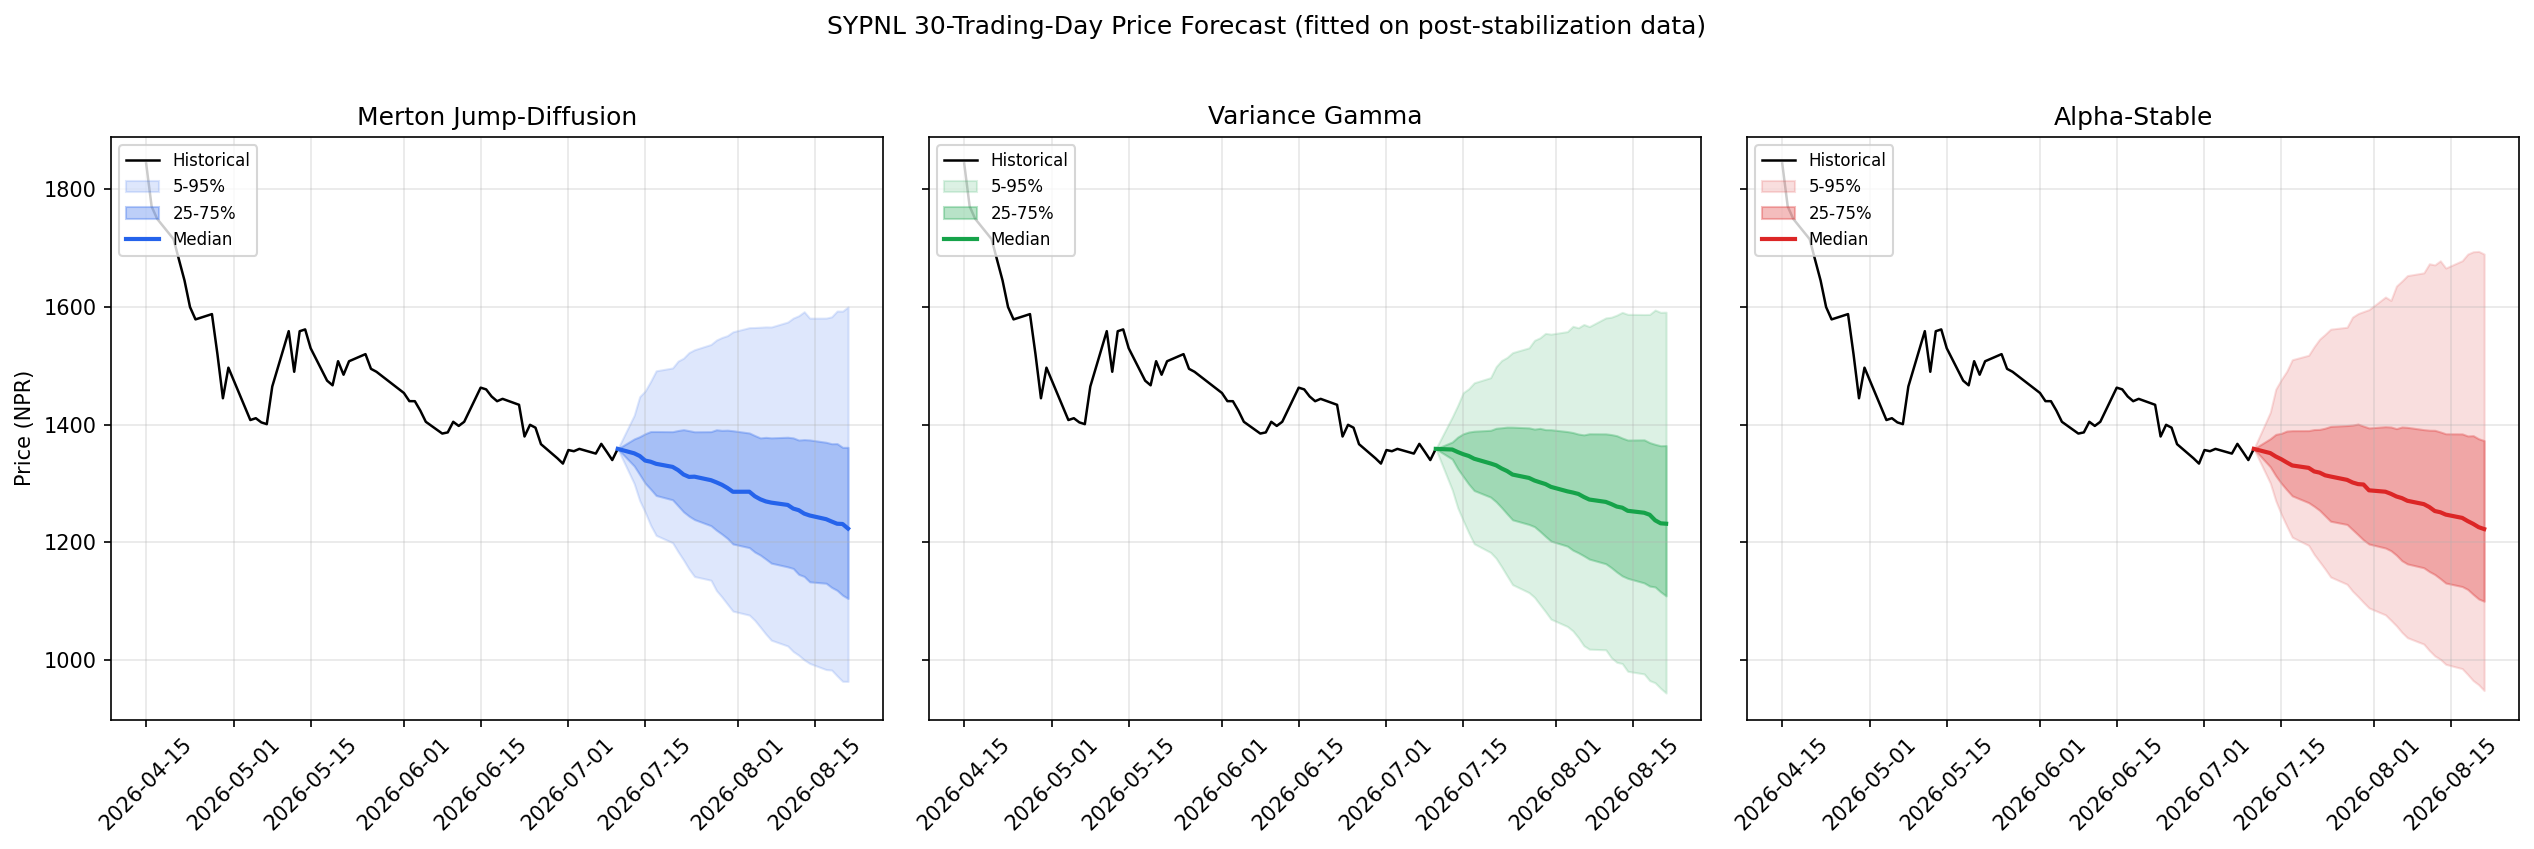
\includegraphics[width=\textwidth]{sypnl_forecast.png}
\caption{30-trading-day price forecast fan charts. Shaded bands show the 25--75\% and 5--95\% ranges of 3{,}000 simulated paths; solid line is the median path.}
\label{fig:forecast}
\end{figure}

\begin{table}[h]
\centering
\small
\begin{tabular}{lrrrrr}
\toprule
Model & p05 & p25 & Median & p75 & p95 \\
\midrule
Merton JD & 964 & 1{,}105 & 1{,}224 & 1{,}362 & 1{,}600 \\
Variance Gamma & 944 & 1{,}109 & 1{,}232 & 1{,}365 & 1{,}591 \\
$\alpha$-Stable & 948 & 1{,}100 & 1{,}223 & 1{,}373 & 1{,}690 \\
\bottomrule
\end{tabular}
\caption{Terminal price distribution (NPR) at $t+30$ trading days.}
\label{tab:summary}
\end{table}

All three models agree closely on the central 50\% of the distribution (25th--75th percentile within $\pm10$ NPR of each other). The models diverge most in the upper tail: the $\alpha$-stable 95th percentile (1{,}690) exceeds the other two by roughly 90--100 NPR, directly reflecting its heavier tail index. The negative median drift relative to the current price reflects the recent downward trend in the post-stabilization sample (SYPNL fell from a March peak near 2{,}000 to the 1{,}300s by July).

\section{Limitations}
\begin{itemize}
\item \textbf{Sample size.} 104 post-stabilization observations is small for pinning down third- and fourth-moment (skew/kurtosis) behavior; standard errors on these calibrated parameters are not reported here but are likely large.
\item \textbf{Merton identifiability.} With only four moment equations available for five parameters, the jump-rate-fixing heuristic is a necessary but somewhat arbitrary simplification; the resulting near-zero $\sigma_J$ suggests the solver found a degenerate rather than a well-separated jump/diffusion decomposition.
\item \textbf{i.i.d.\ assumption.} Lévy processes assume independent, identically distributed increments. SYPNL's price history (the listing rally in particular) shows visible momentum and mean-reversion structure inconsistent with this assumption.
\item \textbf{Non-stationarity risk.} As a stock listed less than eight months ago, SYPNL may not yet trade in a stable statistical regime; parameters fitted today may not hold over the 30-day forecast horizon.
\end{itemize}

\section{Conclusion}
Despite these caveats, the exercise illustrates a core econophysics point: even with a short, noisy sample, standard Lévy models applied to NEPSE data recover return distributions with visibly fatter tails and non-trivial skew relative to the Gaussian benchmark, and the resulting forecast fan charts communicate the width of realistic price uncertainty far more honestly than a single point forecast would.

\section*{References}
\small
\begin{itemize}
\item[] Merton, R.C. (1976). Option pricing when underlying stock returns are discontinuous. \textit{Journal of Financial Economics}, 3(1--2), 125--144.
\item[] Madan, D.B., Carr, P.P., \& Chang, E.C. (1998). The Variance Gamma process and option pricing. \textit{European Finance Review}, 2(1), 79--105.
\item[] Chambers, J.M., Mallows, C.L., \& Stuck, B.W. (1976). A method for simulating stable random variables. \textit{Journal of the American Statistical Association}, 71(354), 340--344.
\item[] Mandelbrot, B. (1963). The variation of certain speculative prices. \textit{Journal of Business}, 36(4), 394--419.
\end{itemize}

\end{document}
